\documentclass[12pt, a4paper, ngerman]{article}

% ── Pakete ──────────────────────────────────────────────────
\usepackage[utf8]{inputenc}
\usepackage[T1]{fontenc}
\usepackage[ngerman]{babel}
\usepackage{lmodern}
\usepackage[left=2.5cm, right=2.5cm, top=2.5cm, bottom=2.5cm]{geometry}
\usepackage{setspace}\onehalfspacing
\usepackage{parskip}

\usepackage{graphicx}
\usepackage{float}
\usepackage{booktabs}
\usepackage{longtable}
\usepackage{listings}
\usepackage{xcolor}
\usepackage{caption}
\usepackage{subcaption}
\usepackage{amsmath}
\usepackage{tikz}
\usepackage{pdflscape}
\usetikzlibrary{arrows.meta, positioning, shapes.geometric, calc}

\usepackage[colorlinks=true, linkcolor=black, citecolor=blue,
            urlcolor=blue]{hyperref}
\usepackage[nottoc]{tocbibind}

\usepackage{fancyhdr}
\setlength{\headheight}{14pt}
\pagestyle{fancy}
\fancyhf{}
\fancyhead[L]{\small Akkuvorhersage mit TinyML}
\fancyhead[R]{\small THWS -- Vertiefung~I}
\fancyfoot[C]{\thepage}
\renewcommand{\headrulewidth}{0.4pt}

\graphicspath{{./}{../reports/figures/}}

% ── THWS Farben ────────────────────────────────────────────
\definecolor{thwsorange}{RGB}{246,130,30}
\definecolor{thwsgrau}{RGB}{90,90,90}

% ── Code-Listings ──────────────────────────────────────────
\definecolor{codebg}{RGB}{248,248,248}
\definecolor{codegreen}{RGB}{40,160,60}
\definecolor{codegray}{RGB}{100,100,100}
\definecolor{codeblue}{RGB}{30,80,180}
\definecolor{codepurple}{RGB}{140,40,140}

\lstdefinestyle{mystyle}{
    backgroundcolor=\color{codebg},
    basicstyle=\ttfamily\footnotesize,
    breakatwhitespace=false,
    breaklines=true,
    captionpos=b,
    commentstyle=\color{codegreen}\itshape,
    keywordstyle=\color{codeblue}\bfseries,
    stringstyle=\color{codepurple},
    numberstyle=\tiny\color{codegray},
    numbers=left,
    numbersep=8pt,
    frame=single,
    rulecolor=\color{codegray!40},
    tabsize=4,
    showstringspaces=false,
    xleftmargin=1.5em,
    framexleftmargin=1em,
}
\lstset{style=mystyle}

\lstdefinelanguage{Kotlin}{
  morekeywords={fun,val,var,class,object,import,package,
                return,if,else,when,for,while,do,in,is,as,
                override,private,public,companion,data,sealed,
                suspend,by,lazy,init,constructor,abstract,
                interface,null,true,false,this,super,try,catch,throw},
  morecomment=[l]{//},
  morecomment=[s]{/*}{*/},
  sensitive=true,
}

% ── Eigene Befehle ─────────────────────────────────────────
\newcommand{\code}[1]{\texttt{#1}}
\newcommand{\datei}[1]{\texttt{\small #1}}

\begin{document}

% ████████████████████████████████████████████████████████████
%  DECKBLATT
% ████████████████████████████████████████████████████████████
\begin{titlepage}
\centering
\vspace*{-1.5cm}

\noindent
\begin{minipage}{0.28\textwidth}
    
\includegraphics[width=\textwidth]{Thws-logo_English.png}
\end{minipage}%
\hfill
\begin{minipage}{0.65\textwidth}
    \raggedleft
    {\Large\textsc{Technische Hochschule\\Würzburg-Schweinfurt}}\\[0.2cm]
    {\large Fakultät Informatik und\\Wirtschaftsinformatik}
\end{minipage}

\vspace{2.5cm}

\rule{\textwidth}{0.6pt}\\[0.5cm]
{\huge\bfseries Entwicklung einer Android-App\\zur Akkuvorhersage mit TinyML}\\[0.4cm]
\rule{\textwidth}{0.6pt}\\[2cm]

{\Large Portfolio-Dokumentation}\\[0.4cm]
{\large Vertiefung I: Mobile und Ubiquitäre Anwendungen}\\[2.5cm]

\begin{tabular}{rl}
\textbf{Vorgelegt von:}    & Keno Schürger \\[0.3em]
\textbf{Matrikelnummer:}   & 5023033 \\[0.3em]
\textbf{Studiengang:}      & Wirtschaftsinformatik (BWI) \\[0.3em]
\textbf{Dozenten:}         & Prof.\ Dr.\ Karsten Huffstadt, \\
                           & Prof.\ Dr.\ Isabel John \\[0.3em]
\textbf{Semester:}         & Sommersemester 2026 \\[0.3em]
\textbf{Bearbeitungszeit:} & 25.\ März -- 11.\ Mai 2026 \\
\end{tabular}

\vfill
{\large Würzburg, \today}
\end{titlepage}

% ████████████████████████████████████████████████████████████
%  VERZEICHNISSE
% ████████████████████████████████████████████████████████████
\pagenumbering{Roman}
\tableofcontents
\newpage
\listoffigures
\listoftables
\lstlistoflistings
\newpage
\pagenumbering{arabic}

% ████████████████████████████████████████████████████████████
%  1  AUSGANGSSITUATION
% ████████████████████████████████████████████████████████████
\section{Ausgangssituation und Motivation}
\label{sec:ausgangssituation}

\subsection{Problemstellung}

Smartphone-Akkuanzeigen funktionieren auf den meisten Geräten seit
Android~5 (2014) nach einem einfachen Prinzip: man rechnet den
durchschnittlichen Verbrauch der letzten Stunden linear in die
Zukunft. Wer schon einmal mit 30\,\% Akku
\glqq{}noch 4 Stunden\grqq{} im Display hatte und dann nach einem
YouTube-Video plötzlich bei 15\,\% mit \glqq{}noch 1 Stunde\grqq{}
stand, kennt das Problem.

Mit Android~12 hat Google im Oktober 2021 ein eigenes
ML-basiertes Modell ins System eingebaut
(\code{PowerManager.getBatteryDischargePrediction()}). Auf
Pixel-Geräten nutzt der Settings-Screen diesen Wert; auf Geräten
anderer Hersteller (Xiaomi, Samsung) wird er meist gar nicht
angezeigt, obwohl die API verfügbar ist.

\subsection{Zielsetzung}

Ziel ist eine Android-App, die

\begin{itemize}
\item alle 30~Sekunden 10~Sensordaten-Features sammelt (Akku,
  Helligkeit, App-Kategorie, CPU, Temperatur usw.),
\item ein eigenes TinyML-Modell on-device einsetzt,
\item parallel die Google-API liest und vergleicht,
\item alles in eine CSV schreibt, die am PC ausgewertet wird.
\end{itemize}

Funktional sollte am Ende stehen:

\begin{enumerate}
\item Eine Android-App, die im Hintergrund Daten sammelt und überlebt
  (Foreground-Service, Auto-Restart nach Boot oder Wegwischen).
\item Ein quantisiertes TFLite-Modell ($<$\,15\,KB), das in der App
  on-device läuft und eine Vorhersage in der Notification anzeigt.
\item Eine Trainings-Pipeline am PC, die die exportierte CSV
  verarbeitet, das Modell trainiert und es zurück in die App
  deployt.
\item Eine Auswertung, die zeigt, wie gut das eigene Modell gegen
  die Google-API und einfache Baselines steht.
\end{enumerate}

Dieses Portfolio dokumentiert den \emph{Bau-Aufwand}, die
Architektur und die Programmier-Eigenleistung. Die
\emph{wissenschaftliche} Auswertung des Multi-Device-Vergleichs ist
Gegenstand der separaten Paper-Einreichung
(\datei{paper/main.pdf} im selben Repo).

\subsection{Rahmenbedingungen}

\begin{itemize}
\item \textbf{Eigenes Gerät:} Xiaomi 2107113SG (Redmi Note 10 Pro),
  Android 12, 8\,GB RAM.
\item \textbf{Zusätzliche Test-Geräte} (Mitstudierende): Google
  Pixel~7~Pro, Pixel~8~Pro, Pixel~9~Pro~XL.
\item \textbf{Entwicklungsumgebung:} Android Studio (Kotlin),
  Python 3.13 mit TensorFlow 2.21 am Windows-Notebook.
\item \textbf{Bearbeitungszeitraum:} 25.\ März bis 11.\ Mai 2026
  (sieben Wochen).
\end{itemize}

\newpage

% ████████████████████████████████████████████████████████████
%  2  ARCHITEKTURMODELL
% ████████████████████████████████████████████████████████████
\section{Architekturmodell}
\label{sec:architektur}

\subsection{Gesamtarchitektur im Überblick}

Das System gliedert sich in zwei klar getrennte Hälften, die durch
CSV-Dateien und das \datei{.tflite}-Modell als Schnittstellen
kommunizieren:

\begin{enumerate}
\item \textbf{Datenerhebung (Android-App)} -- alle 30 Sekunden ein
  Datenpunkt mit 10 Features, gespeichert in CSV.
\item \textbf{Modelltraining (Python-Pipeline)} -- liest die
  konsolidierte CSV, trainiert Conv1D, konvertiert nach TFLite.
\item \textbf{On-Device-Inferenz (Android-App)} -- das TFLite-Modell
  läuft direkt im Phone und liefert die Vorhersage in der
  Notification.
\end{enumerate}

\begin{figure}[H]
\centering
\begin{tikzpicture}[
    node distance=2.8cm,
    box/.style={
        rectangle, draw, rounded corners=4pt,
        minimum height=1.4cm, minimum width=3cm,
        text width=2.8cm, align=center,
        font=\small\bfseries,
        fill=thwsorange!10
    },
    arrow/.style={
        -{Stealth[length=3mm]}, thick, thwsgrau
    },
    lbl/.style={
        font=\footnotesize, midway, above, text=black
    },
    sub/.style={
        font=\footnotesize\itshape, text=gray!70!black
    }
]

\node[box] (app1) {Android-App};
\node[sub, below=0.1cm of app1] {(Datensammlung)};

\node[box, right=of app1] (python) {Python-Pipeline};
\node[sub, below=0.1cm of python, text width=3cm, align=center]
    {(Training, Auswertung)};

\node[box, right=of python] (app2) {Android-App};
\node[sub, below=0.1cm of app2, text width=3cm, align=center]
    {(On-Device-Inferenz)};

\draw[arrow] (app1) -- node[lbl] {CSV-Export} (python);
\draw[arrow] (python) -- node[lbl] {.tflite + Scaler} (app2);

\end{tikzpicture}
\caption{Vereinfachter Datenfluss zwischen den Systemkomponenten}
\label{fig:datenfluss}
\end{figure}

Die vollständige Detail-Architektur mit allen Unterkomponenten,
internen Verbindungen und Schnittstellen zeigt
Abbildung~\ref{fig:architektur_gesamt} auf der folgenden Seite.

\begin{landscape}
\thispagestyle{empty}
\vspace*{\fill}
\begin{figure}[H]
    \centering
    
\includegraphics[width=\linewidth,height=0.82\textheight,keepaspectratio]{architektur_gesamt1.png}
    \caption{Detaillierte Gesamtarchitektur des Battery-Predictor-Systems}
    \label{fig:architektur_gesamt}
\end{figure}
\vspace*{\fill}
\end{landscape}

\subsection{Android-App im Detail}

Die App ist in sechs Kotlin-Dateien gegliedert:

\begin{table}[H]
\centering
\caption{Module der Android-App}
\label{tab:android_module}
\begin{tabular}{lp{9cm}}
\toprule
\textbf{Datei} & \textbf{Aufgabe} \\
\midrule
\datei{MainActivity.kt}        & UI mit Start/Stopp/Export-Buttons, zeigt aktuelle Vorhersage \\
\datei{DataCollectorService.kt}& Foreground-Service, sammelt alle 30 Sekunden Daten \\
\datei{BatteryDataPoint.kt}    & Datenklasse für einen Messpunkt mit CSV-Serialisierung \\
\datei{BatteryDataLogger.kt}   & Schreibt CSV in \code{filesDir}, behandelt Schema-Drift \\
\datei{BatteryPredictor.kt}    & TFLite-Interpreter mit StandardScaler-Normalisierung \\
\datei{BootReceiver.kt}        & Startet den Service nach Geräte-Neustart \\
\bottomrule
\end{tabular}
\end{table}

\subsection{Python-Pipeline im Detail}

Die Auswerte-Seite ist nach \emph{Forschungs-Methodik} organisiert
(eigener Ordner pro Methode, separater Eval-Ordner). Der Orchestrator
\datei{run\_pipeline.py} bringt sie in Reihenfolge:

\begin{enumerate}
\item \datei{methods/tinyml/merge\_devices.py} -- alle Geräte-CSVs zu
  einer kombinierten CSV zusammenführen
\item \datei{methods/tinyml/data\_prep.py} -- Discharge-Segmente
  finden, Sliding-Windows bilden, Segment-Level-Split
\item \datei{methods/tinyml/train.py} -- Conv1D-Modell trainieren
\item \datei{methods/tinyml/tflite\_convert.py} -- Konvertierung in
  drei TFLite-Varianten (dynamic, float16, int8)
\item \datei{methods/*/predict.py} -- Vorhersagen aller sechs
  verglichenen Methoden auf dem Test-Set
\item \datei{evaluation/*.py} -- diverse Auswertungs-Skripte
\end{enumerate}

\newpage

% ████████████████████████████████████████████████████████████
%  3  DATENMODELL
% ████████████████████████████████████████████████████████████
\section{Datenmodell}
\label{sec:datenmodell}

\subsection{CSV-Schema}

Pro Messpunkt schreibt die App eine Zeile mit folgenden Spalten:

\begin{table}[H]
\centering
\caption{Felder eines CSV-Eintrags}
\label{tab:csv_schema}
\small
\begin{tabular}{lll}
\toprule
\textbf{Spalte} & \textbf{Typ} & \textbf{Bedeutung} \\
\midrule
\code{session\_id}         & String (8) & Zufalls-ID pro Service-Start \\
\code{timestamp}           & long (ms)  & Unix-Zeitstempel \\
\code{datetime}            & String     & YYYY-MM-DD HH:MM:SS \\
\midrule
\code{battery\_level}      & Float 0--100 & Akku-Stand in Prozent \\
\code{screen\_on}          & Int 0/1      & Bildschirm an? \\
\code{brightness}          & Float 0--100 & Helligkeit normalisiert \\
\code{active\_app\_category}& Int 0--5    & 0=idle, 1=social, 2=video, 3=gaming, 4=browser, 5=productivity \\
\code{wifi\_on}            & Int 0/1      & WiFi-verbunden? \\
\code{mobile\_data\_on}    & Int 0/1      & Mobilfunk aktiv? \\
\code{charging}            & Int 0/1      & Lädt gerade? \\
\code{cpu\_usage}          & Float 0--100 & CPU-Frequenz-Auslastung (Proxy) \\
\code{temperature}         & Float (°C)   & Akku-Temperatur \\
\code{hotspot\_on}         & Int 0/1      & WLAN-Hotspot aktiv? \\
\midrule
\code{system\_estimate\_min}& Float       & Google-API-Schätzung in Minuten \\
\code{system\_personalized}& Int $-$1/0/1 & Ist Google-Schätzung gerätspezifisch? \\
\code{own\_prediction\_h}  & Float        & Eigene TinyML-Vorhersage (Stunden) \\
\code{linear\_baseline\_h} & Float        & Naive Vorhersage aus BatteryManager-Countern \\
\bottomrule
\end{tabular}
\end{table}

Die ersten drei Spalten sind Metadaten, die zehn nächsten sind die
\emph{Features} für das ML-Modell, die letzten vier sind
Vergleichswerte zur Auswertung.

\subsection{Warum genau diese zehn Features?}

Bei der Auswahl gab es eine harte Regel: \emph{ich darf nur lesen,
was eine normale App ohne Spezial-Berechtigung lesen kann.} Damit
fielen einige naheliegende Kandidaten weg:

\begin{itemize}
\item \textbf{Genaue Stromstärke pro App} (PowerStats HAL): nur
  System-Apps.
\item \textbf{Battery Health} (Verschleißzustand): teilweise gesperrt.
\item \textbf{Kernel-Fuel-Gauge}: gesperrt.
\end{itemize}

Was übrig blieb, sind die zehn Features oben. Sie decken drei
Gruppen ab: \textbf{Akkuzustand} (level, temperature, charging),
\textbf{Nutzungsintensität} (screen, brightness, app\_category,
cpu\_usage), \textbf{Konnektivität} (wifi, mobile, hotspot).

\subsection{Speicherung und Export}

Die CSV liegt im app-internen Verzeichnis
(\code{Context.filesDir}). Das ist nur für diese App lesbar -- weder
andere Apps noch ein angeschlossener PC können die Datei direkt
sehen (siehe Kapitel~\ref{sec:datenschutz}). Der Export erfolgt
explizit per Share-Intent durch den Nutzer.

Über vier Geräte hinweg wurden in 45 Tagen
\textbf{66.001 Messpunkte} in \textbf{180 Sessions} gesammelt.

\subsection{Die App in Aktion}

Abbildung~\ref{fig:app_screenshots} zeigt die Main Activity der App
auf dem Xiaomi 2107113SG zu zwei Zeitpunkten: einmal direkt nach
dem Service-Start (Modell sammelt erst zehn Datenpunkte, also
fünf Minuten Aufwärmphase) und einmal mit aktiver TinyML-Vorhersage.
Der Datenpunkt-Zähler im unteren Bereich (\code{Gesammelte
Datenpunkte: 47\,572}) ist ein wichtiges UX-Element: er gibt dem
Nutzer Feedback, dass der Service tatsächlich noch läuft, ohne dass
er die Notification öffnen muss.

\begin{figure}[H]
\centering
\begin{subfigure}{0.42\textwidth}
    \centering
    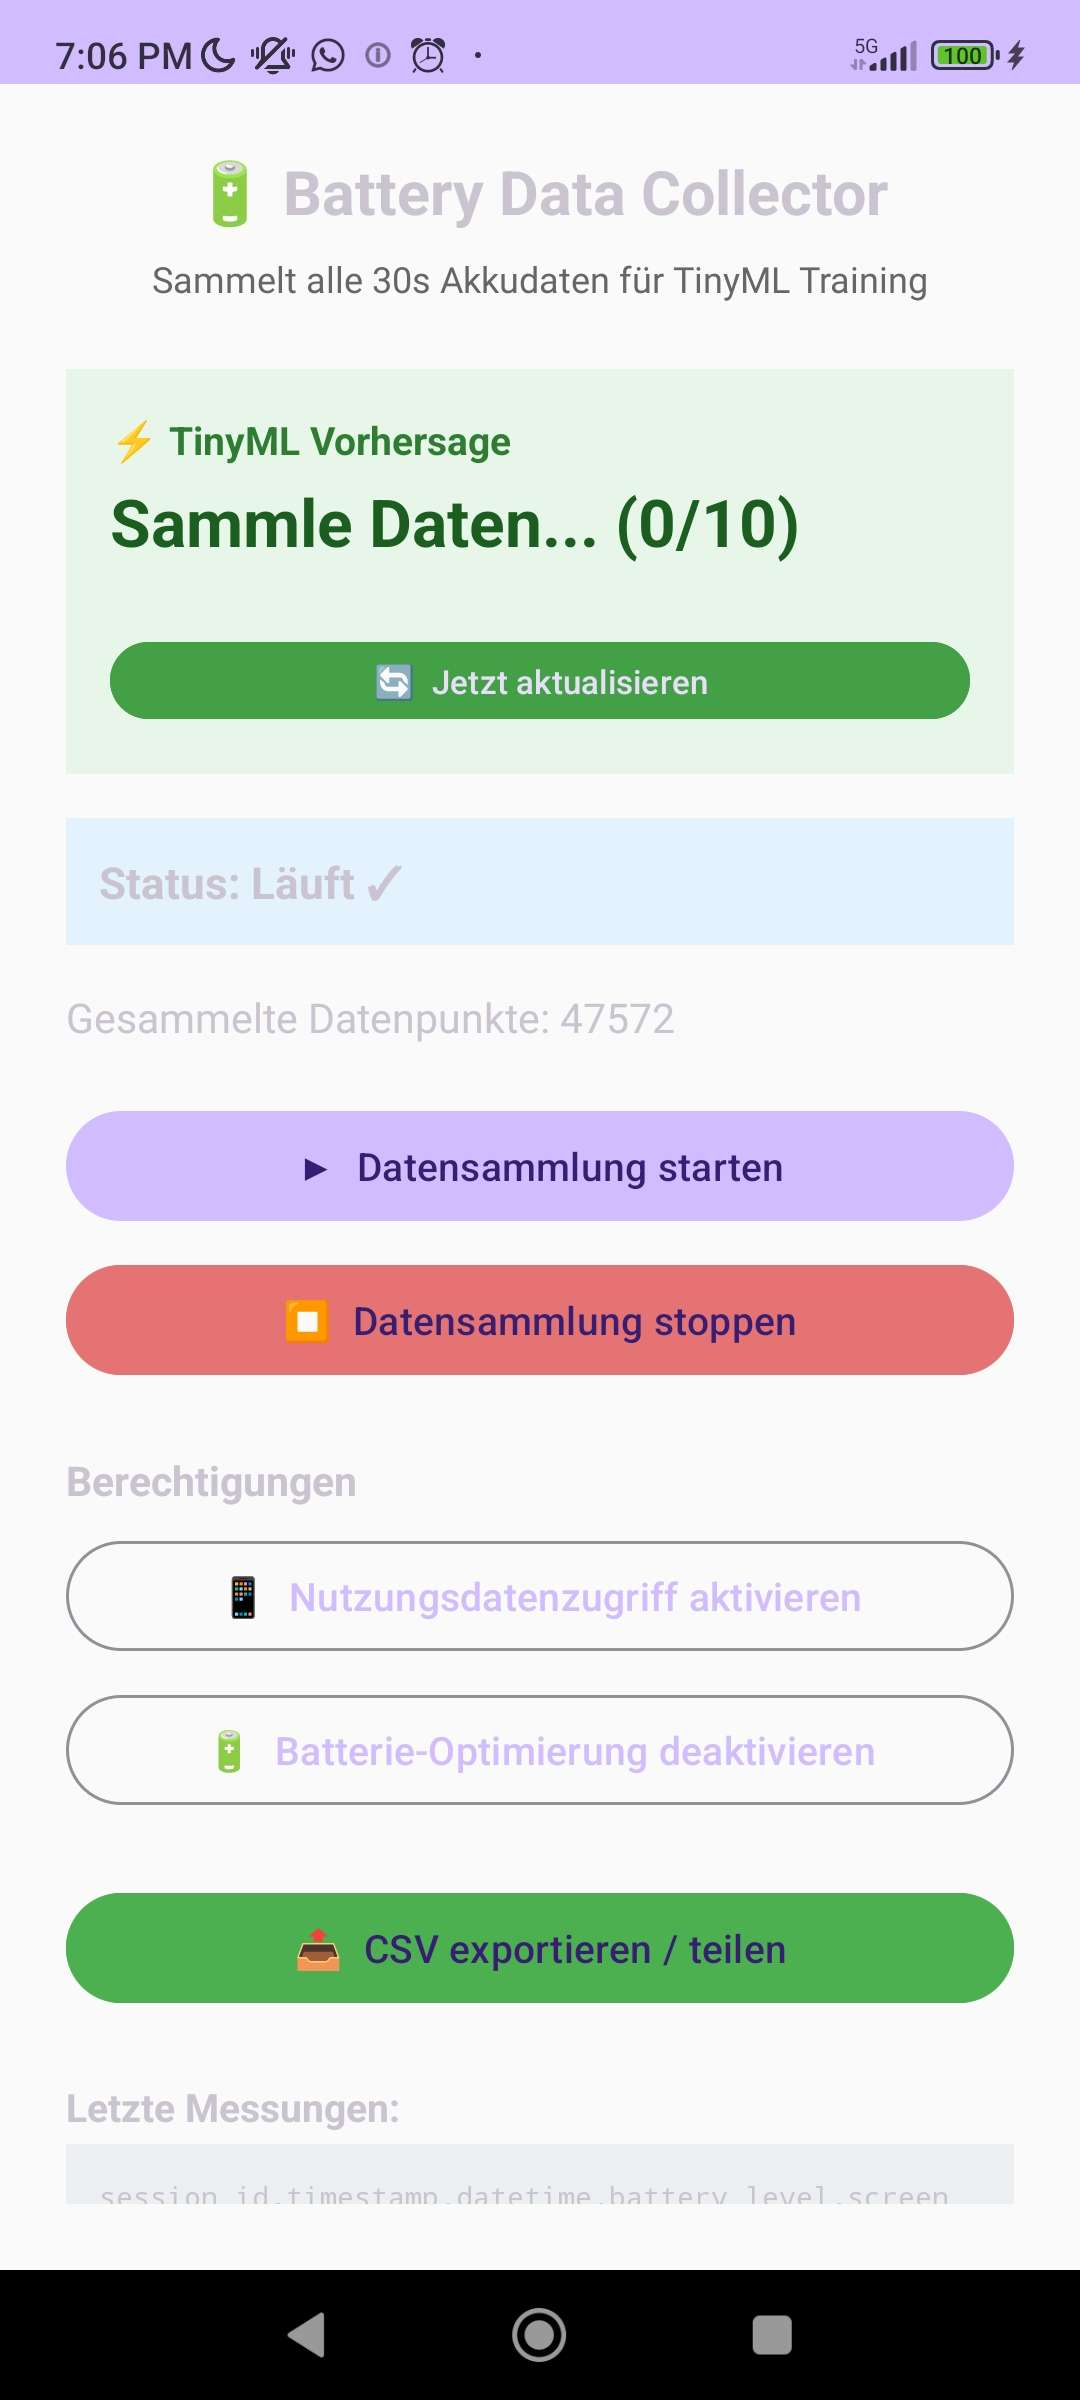
\includegraphics[width=\linewidth]{screenshot_app_start.jpg}
    \caption{Aufwärmphase: \glqq{}Sammle Daten\ldots\ (0/10)\grqq{}.
    Bis zehn Messpunkte vorliegen, gibt das Modell noch keine
    Vorhersage aus.}
    \label{fig:app_start}
\end{subfigure}\hfill
\begin{subfigure}{0.42\textwidth}
    \centering
    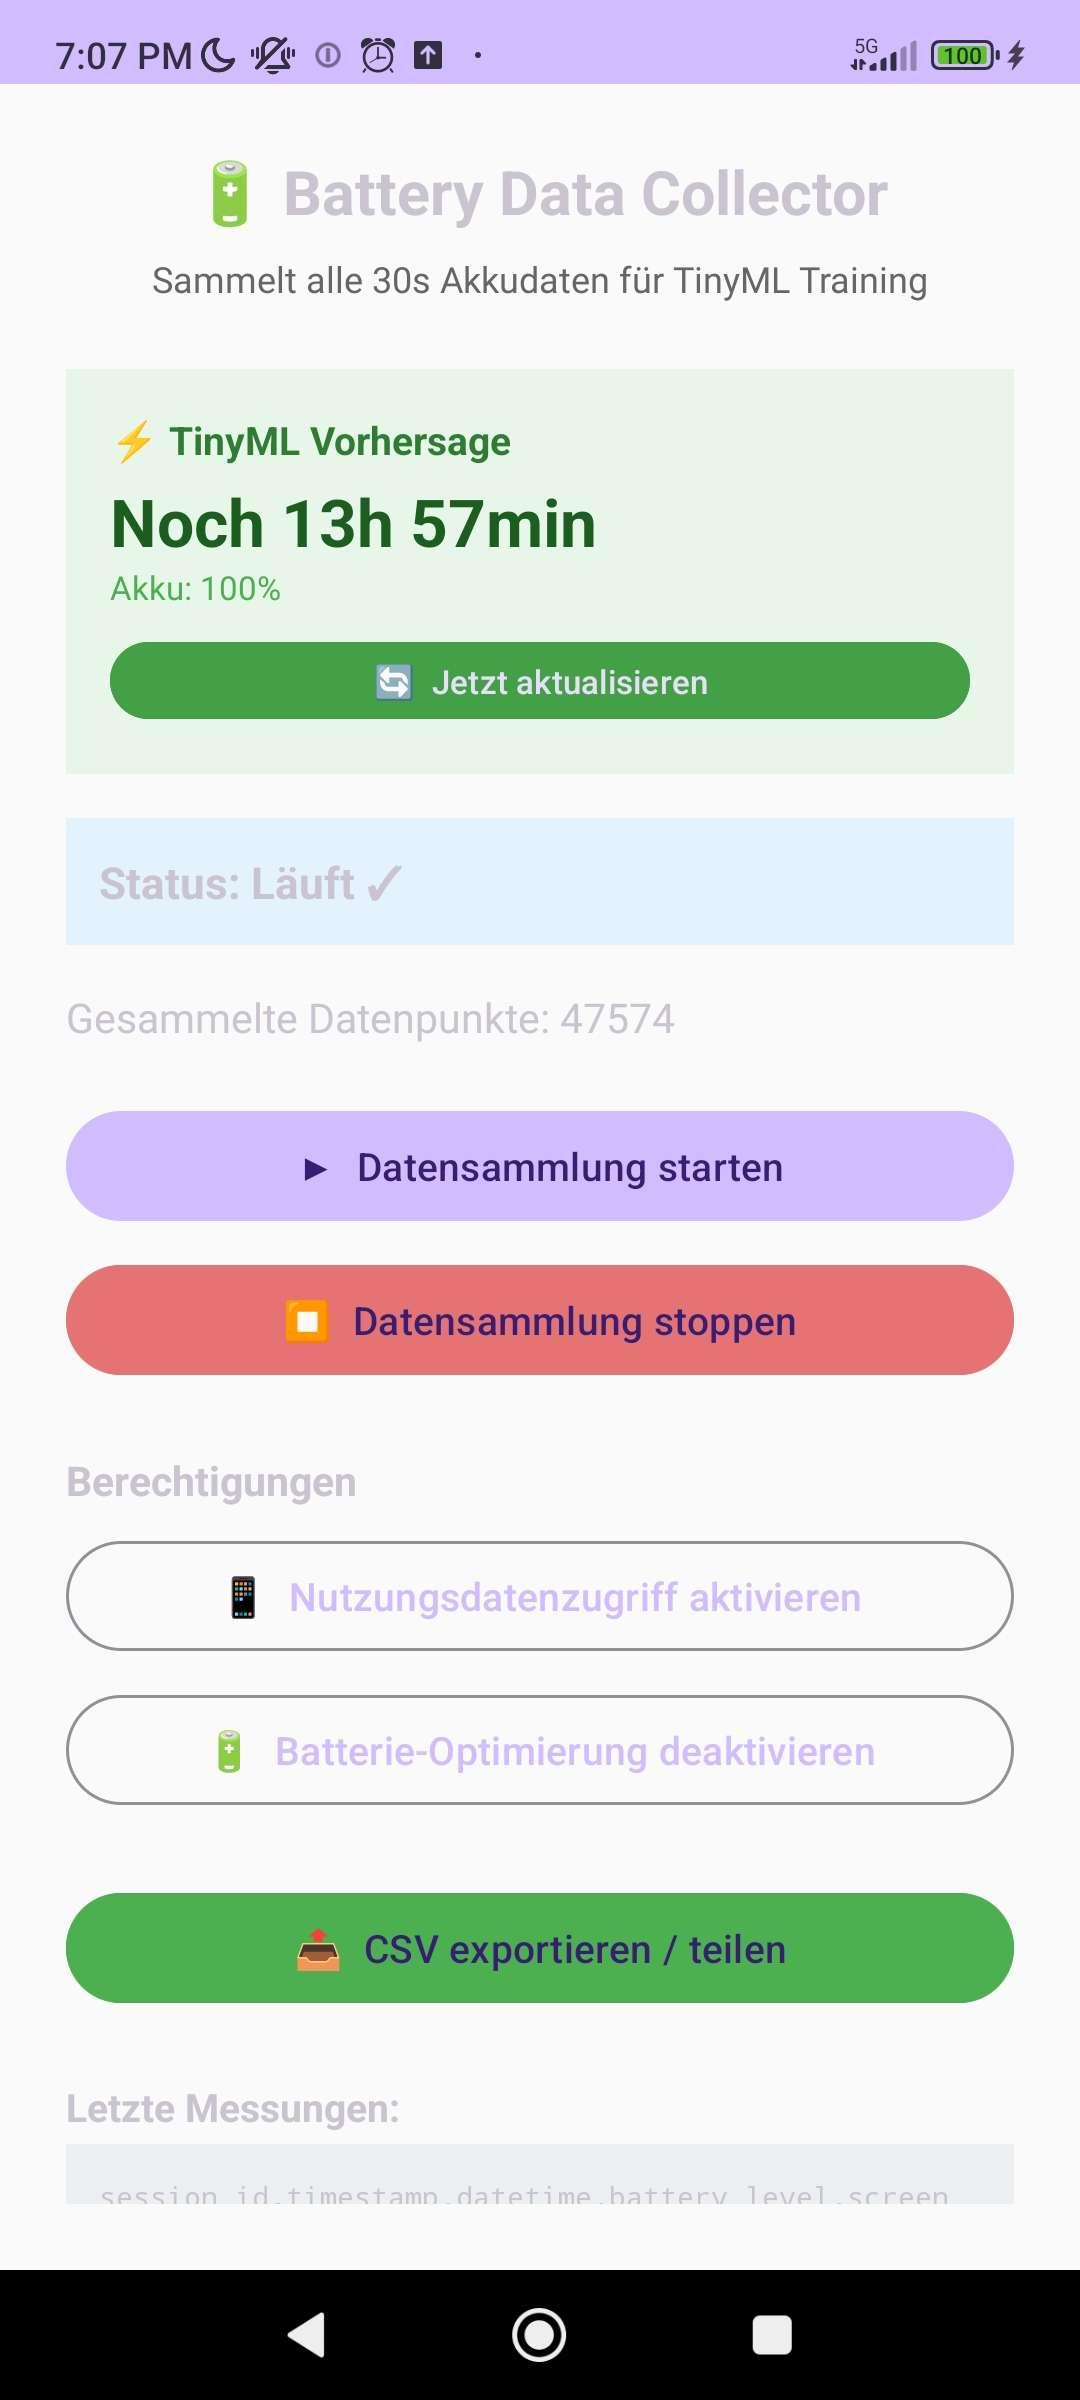
\includegraphics[width=\linewidth]{screenshot_app_prediction.jpg}
    \caption{Aktive Vorhersage: \glqq{}Noch 13\,h 57\,min\grqq{}
    bei 100\,\% Akku. Die TinyML-Inferenz läuft direkt auf dem
    Phone.}
    \label{fig:app_prediction}
\end{subfigure}
\caption{Main Activity der Battery Data Collector App auf dem
Xiaomi 2107113SG (Redmi Note 10 Pro). Links: erste Sekunden nach
Service-Start. Rechts: dasselbe Gerät eine Minute später mit fertiger
On-Device-Vorhersage.}
\label{fig:app_screenshots}
\end{figure}

\newpage

% ████████████████████████████████████████████████████████████
%  4  PROGRAMMIERUNG
% ████████████████████████████████████████████████████████████
\section{Programmierung}
\label{sec:programmierung}

\subsection{Datensammlung im Service}

Der Kern des \code{DataCollectorService} ist ein
\code{Handler.postDelayed}-Loop, der alle 30 Sekunden eine Messung
auslöst:

\begin{lstlisting}[language=Kotlin,caption={Mess-Schleife im DataCollectorService}]
private val INTERVAL_MS = 30 * 1000L  // 30 Sekunden

private val collectRunnable = object : Runnable {
    override fun run() {
        collectAndLog()
        handler.postDelayed(this, INTERVAL_MS)
    }
}

private fun collectAndLog() {
    // 1) Roh-Features lesen
    val batteryLevel = getBatteryLevel()
    val screenOn = if (isScreenOn()) 1 else 0
    val brightness = getScreenBrightness()
    // ... (10 Features insgesamt)

    // 2) TinyML-Vorhersage (fail-safe)
    val features = floatArrayOf(batteryLevel, screenOn.toFloat(), /* ... */)
    var prediction = -1f
    try {
        predictor?.let { prediction = it.addDataAndPredict(features) }
    } catch (e: Exception) {
        Log.e("BatteryCollector", "Prediction failed: ${e.message}")
    }

    // 3) Vergleichswerte einlesen
    val systemEstimateMin = getSystemBatteryEstimate()
    val linearBaselineH = getLinearBaselineHours()

    // 4) Datenpunkt schreiben
    logger.log(BatteryDataPoint(/* ... */), sessionId)
}
\end{lstlisting}

\subsection{Auslesen der 10 Features}

Die meisten Werte kommen direkt aus den Android-System-Services.
Drei Sachen waren tricky.

\subsubsection*{CPU-Auslastung}

Seit Android 8 ist \code{/proc/stat} für Apps gesperrt. Statt der
\glqq{}echten\grqq{} CPU-Auslastung lese ich die aktuelle
CPU-Frequenz pro Kern und vergleiche mit der Maximalfrequenz.
Höhere Frequenz = höhere Last:

\begin{lstlisting}[language=Kotlin,caption={CPU-Last als Frequenz-Proxy}]
private fun getAvgCpuFrequencyPercent(): Float {
    val numCores = Runtime.getRuntime().availableProcessors()
    var totalRatio = 0f
    var readCores = 0
    for (i in 0 until numCores) {
        try {
            val cur = File("/sys/devices/system/cpu/cpu$i/cpufreq/scaling_cur_freq")
                .readText().trim().toLong()
            val max = File("/sys/devices/system/cpu/cpu$i/cpufreq/cpuinfo_max_freq")
                .readText().trim().toLong()
            if (max > 0) {
                totalRatio += cur.toFloat() / max
                readCores++
            }
        } catch (_: Exception) { }
    }
    if (readCores == 0) throw Exception("No CPU freq readable")
    return (totalRatio / readCores * 100f).coerceIn(0f, 100f)
}
\end{lstlisting}

\subsubsection*{Aktive App}

Mit dem \code{UsageStatsManager} (Permission
\code{PACKAGE\_USAGE\_STATS}, die der Nutzer manuell in den
Einstellungen aktivieren muss) lese ich die zuletzt benutzte App
und ordne sie über ein Package-Prefix-Mapping einer Kategorie zu:

\begin{lstlisting}[language=Kotlin,caption={App-Kategorisierung (Auszug)}]
private val APP_CATEGORIES = mapOf(
    "com.instagram"           to 1, // social
    "com.whatsapp"            to 1,
    "org.telegram"            to 1,
    "com.google.android.youtube" to 2, // video
    "com.netflix"             to 2,
    "com.spotify"             to 2,
    "com.supercell"           to 3, // gaming
    "com.miHoYo"              to 3,
    "com.google.android.apps.chrome" to 4, // browser
    "org.mozilla"             to 4,
    "com.google.android.apps.docs"   to 5, // productivity
    "com.microsoft"           to 5,
    // ... (rund 30 Eintraege)
)
\end{lstlisting}

Unbekannte Packages bekommen Kategorie 0 (idle), werden aber
zusätzlich geloggt, damit ich sie später nachmappen kann.

\subsubsection*{Hotspot-Status}

Die offizielle \code{WifiManager.isWifiApEnabled()}-API ist als
\code{@hide} markiert, also nicht im SDK. Über Reflection ist sie
trotzdem erreichbar:

\begin{lstlisting}[language=Kotlin,caption={Hotspot-Status via Reflection}]
private fun isHotspotOn(): Boolean {
    return try {
        val wm = applicationContext.getSystemService(Context.WIFI_SERVICE) as WifiManager
        val method = wm.javaClass.getDeclaredMethod("isWifiApEnabled")
        method.isAccessible = true
        method.invoke(wm) as Boolean
    } catch (e: Exception) {
        false
    }
}
\end{lstlisting}

\subsection{On-Device-Inferenz mit TFLite}

Der \code{BatteryPredictor} hält das TFLite-Modell und einen
Ringpuffer mit den letzten 10 Datenpunkten. Erst wenn der Puffer
voll ist, wird vorhergesagt. Wichtig: die Features müssen mit
denselben StandardScaler-Werten normalisiert werden, mit denen das
Modell trainiert wurde -- die Werte sind hardcoded in der App und
werden bei jedem Re-Training neu hineingeschrieben.

\begin{lstlisting}[language=Kotlin,caption={Inferenz mit TFLite}]
class BatteryPredictor(context: Context) {
    companion object {
        const val SEQUENCE_LENGTH = 10
        const val NUM_FEATURES = 10
        // Werte aus models/scaler.joblib (Multi-Device-Training)
        private val SCALER_MEAN = floatArrayOf(
            68.79f, 0.83f, 8.47f, 1.31f, 0.08f,
            0.92f, 0.00f, 46.35f, 33.00f, 0.07f
        )
        private val SCALER_SCALE = floatArrayOf(
            29.61f, 0.38f, 13.01f, 1.17f, 0.27f,
            0.27f, 1.00f, 16.93f, 4.21f, 0.26f
        )
    }
    private val interpreter: Interpreter
    private val recentData = ArrayDeque<FloatArray>(SEQUENCE_LENGTH)

    fun addDataAndPredict(features: FloatArray): Float {
        val normalized = FloatArray(NUM_FEATURES) { i ->
            (features[i] - SCALER_MEAN[i]) / SCALER_SCALE[i]
        }
        if (recentData.size >= SEQUENCE_LENGTH) recentData.removeFirst()
        recentData.addLast(normalized)
        if (recentData.size < SEQUENCE_LENGTH) return -1f

        val input = ByteBuffer.allocateDirect(SEQUENCE_LENGTH * NUM_FEATURES * 4)
            .order(ByteOrder.nativeOrder())
        for (step in recentData) for (v in step) input.putFloat(v)
        val output = ByteBuffer.allocateDirect(4).order(ByteOrder.nativeOrder())
        interpreter.run(input, output)
        output.rewind()
        return output.float.coerceAtLeast(0f)
    }
}
\end{lstlisting}

\subsection{Robustheit -- die App muss überleben}

Das war der frustrierendste Teil. Android killt Hintergrund-Services
aggressiv, gerade auf Xiaomi-Geräten mit MIUI-Aufsatz. Drei
Mechanismen sorgen dafür, dass die Datensammlung nicht abreißt:

\begin{enumerate}
\item \textbf{Foreground-Service} mit dauerhafter Notification.
\item \textbf{Auto-Restart nach Wegwischen} der App-Karte. Wenn der
  Nutzer die App in der Übersicht wegwischt, registriert sich der
  Service über \code{AlarmManager.setExactAndAllowWhileIdle()}
  einen Restart in 1 Sekunde.
\item \textbf{Auto-Restart nach Geräte-Neustart} über einen
  \code{BootReceiver}, der das \code{BOOT\_COMPLETED}-Intent
  abfängt -- aber nur, wenn der Nutzer den Sammler explizit
  aktiviert hatte.
\end{enumerate}

\begin{lstlisting}[language=Kotlin,caption={Auto-Restart bei onTaskRemoved}]
override fun onTaskRemoved(rootIntent: Intent?) {
    val restartIntent = Intent(this, DataCollectorService::class.java)
    val pendingIntent = PendingIntent.getService(
        this, 99, restartIntent,
        PendingIntent.FLAG_ONE_SHOT or PendingIntent.FLAG_IMMUTABLE
    )
    val alarm = getSystemService(Context.ALARM_SERVICE) as AlarmManager
    alarm.setExactAndAllowWhileIdle(
        AlarmManager.ELAPSED_REALTIME_WAKEUP,
        SystemClock.elapsedRealtime() + 1000,
        pendingIntent
    )
    super.onTaskRemoved(rootIntent)
}
\end{lstlisting}

\subsection{Schema-Drift im Logger}

Beim Hinzufügen neuer Spalten (etwa \code{system\_personalized}
oder \code{linear\_baseline\_h}) hatten bestehende CSV-Dateien
weniger Spalten als die neue Version erwartete. Der Logger prüft
deshalb beim Start die Header-Zeile und parkt alte CSVs automatisch:

\begin{lstlisting}[language=Kotlin,caption={Schema-Drift im Logger abfangen}]
init {
    val expectedHeader = "session_id,timestamp,datetime,${BatteryDataPoint.CSV_HEADER}"
    if (!csvFile.exists() || csvFile.length() == 0L) {
        csvFile.writeText("$expectedHeader\n")
    } else {
        val firstLine = csvFile.useLines { it.firstOrNull() ?: "" }
        if (firstLine != expectedHeader) {
            val backup = File(context.filesDir,
                "battery_data_legacy_${System.currentTimeMillis()}.csv")
            csvFile.copyTo(backup, overwrite = true)
            csvFile.writeText("$expectedHeader\n")
        }
    }
}
\end{lstlisting}

\subsection{Python-Pipeline -- Beispiel Segment-Erkennung}

Die wichtigste Pipeline-Funktion findet Entlade-\emph{Segmente}:
zusammenhängende Phasen, in denen das Phone entladen wird, ohne
zwischendurch zu laden. Daraus werden später Sliding-Window-Sequenzen
gebildet.

\begin{lstlisting}[language=Python,caption={Discharge-Segmente finden}]
def find_discharge_segments(df, min_length, max_gap_ms):
    segments = []
    for _, session_df in df.groupby("session_id"):
        session_df = session_df.sort_values("timestamp").reset_index(drop=True)
        is_discharging = session_df["charging"] == 0
        block_id = (~is_discharging).cumsum()  # neuer Block bei Laden
        for _, block in session_df[is_discharging].groupby(block_id[is_discharging]):
            # innerhalb des Blocks bei groesseren Zeitluecken splitten
            time_diffs = block["timestamp"].diff()
            gap_id = (time_diffs > max_gap_ms).cumsum()
            for _, sub in block.groupby(gap_id):
                if len(sub) >= min_length:
                    segments.append(sub.reset_index(drop=True).copy())
    return segments
\end{lstlisting}

\subsection{Trainings-Verlauf}

Abbildung~\ref{fig:training_curves} zeigt den Trainings- und
Validierungs-Verlauf des Conv1D-Modells über die 21~Epochen, nach
denen EarlyStopping greift.

\begin{figure}[H]
\centering
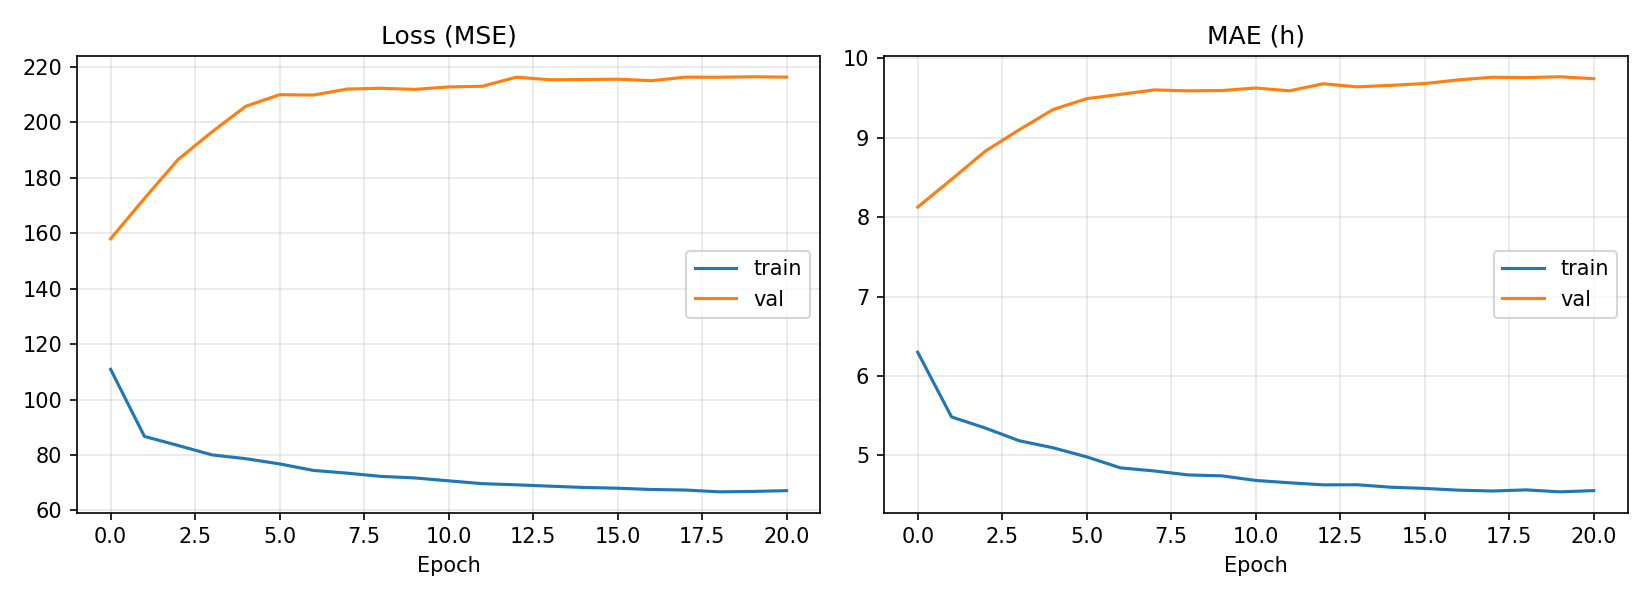
\includegraphics[width=0.8\linewidth]{training_curves.png}
\caption{Trainings- und Validation-MAE des Conv1D-Modells.
Auf dem Multi-Device-Datensatz erreicht das Modell nach
21~Epochen ein Validation-MAE von ca.\ 8\,h. Da
EarlyStopping mit \code{restore\_best\_weights=True}
konfiguriert ist, wird das beste Modell zurückgegeben.}
\label{fig:training_curves}
\end{figure}

\newpage

% ████████████████████████████████████████████████████████████
%  5  EIGENLEISTUNG
% ████████████████████████████████████████████████████████████
\section{Eigenleistung}
\label{sec:eigenleistung}

Im Repo liegen aktuell folgende Code-Mengen:

\begin{table}[H]
\centering
\caption{Code-Umfang nach Bereich}
\label{tab:codeumfang}
\begin{tabular}{lr}
\toprule
\textbf{Bereich} & \textbf{Zeilen (ohne Leerzeilen)} \\
\midrule
Android-App (6 Kotlin-Dateien)                       & $\approx$\;750 \\
Python-Pipeline (\code{methods/}, 12 Module)         & $\approx$\;1{,}050 \\
Python-Auswertung (\code{evaluation/}, 11 Module)    & $\approx$\;1{,}200 \\
Konfiguration und Orchestrator                       & $\approx$\;200 \\
\midrule
\textbf{Summe}                                       & \textbf{$\approx$\;3{,}200} \\
\bottomrule
\end{tabular}
\end{table}

\subsection{Was selbst geschrieben wurde}

\begin{itemize}
\item Gesamte Android-App-Struktur (Activity, Service,
  BroadcastReceiver, FileProvider), inklusive
  \code{onTaskRemoved}-Auto-Restart und Schema-Drift-Detection.
\item Auswahl und Implementierung der zehn Features
  (CPU-Frequenz-Proxy, App-Kategorie-Mapping, Hotspot-Reflection).
\item Datenmodell, CSV-Schema und FileProvider-Konfiguration für
  den Share-Export.
\item Pipeline-Architektur (sechs verglichene Methoden je eigenes
  Modul, Trennung von Methoden- und Auswertungs-Schicht).
\item Konkrete Implementierung der analytischen Baselines (Linear,
  Exponential mit Fallback und Cap gegen Divergenz).
\item Segment-Level-Split als Anti-Leakage-Mechanismus -- der
  vermutlich wichtigste methodische Beitrag.
\item Auswertungs-Skripte: Bootstrap-Konfidenzintervalle,
  Permutationstests, Per-Device-Analyse, Per-Bucket-Analyse.
\end{itemize}

\subsection{Was übernommen wurde}

\begin{itemize}
\item Conv1D-Architektur in Anlehnung an gängige TinyML-Topologien
  (zwei Convolutions, GlobalAveragePooling, zwei Dense).
\item TFLite-Konvertierungs-API (Standard-Funktionen von TensorFlow).
\item \code{scikit-learn}: \code{StandardScaler},
  \code{RandomForestRegressor}, \code{train\_test\_split}.
\item \code{scipy}: \code{curve\_fit} für den exponentiellen Fit.
\end{itemize}

\subsection{Probleme und wie sie gelöst wurden}

\begin{itemize}
\item \emph{Service stirbt auf MIUI:} Auto-Restart über AlarmManager.
\item \emph{\code{/proc/stat} gesperrt:} Frequenz-Proxy statt echter
  Auslastung.
\item \emph{CSV-Schema-Migration:} Header-Check beim Service-Start.
\item \emph{TinyML auf Single-Device zeigt MAE 0.5\,h Artefakt:}
  Segment-Level-Split eingeführt, korrigiert den scheinbaren Wert
  auf 9.96\,h.
\item \emph{Exponential-Fit divergiert manchmal in 30.000\,h:}
  72-h-Cap als Sanity-Bound.
\end{itemize}

\subsection{Ergebnis-Visualisierung}

Abbildung~\ref{fig:cumulative} zeigt die kumulative Fehlerverteilung
auf dem Test-Set für alle sechs verglichenen Methoden -- bei einer
Toleranz von 2\,h erreichen die Top-Methoden (Linear, Exp,
Google-API) rund 60\,\% Trefferquote.

\begin{figure}[H]
\centering
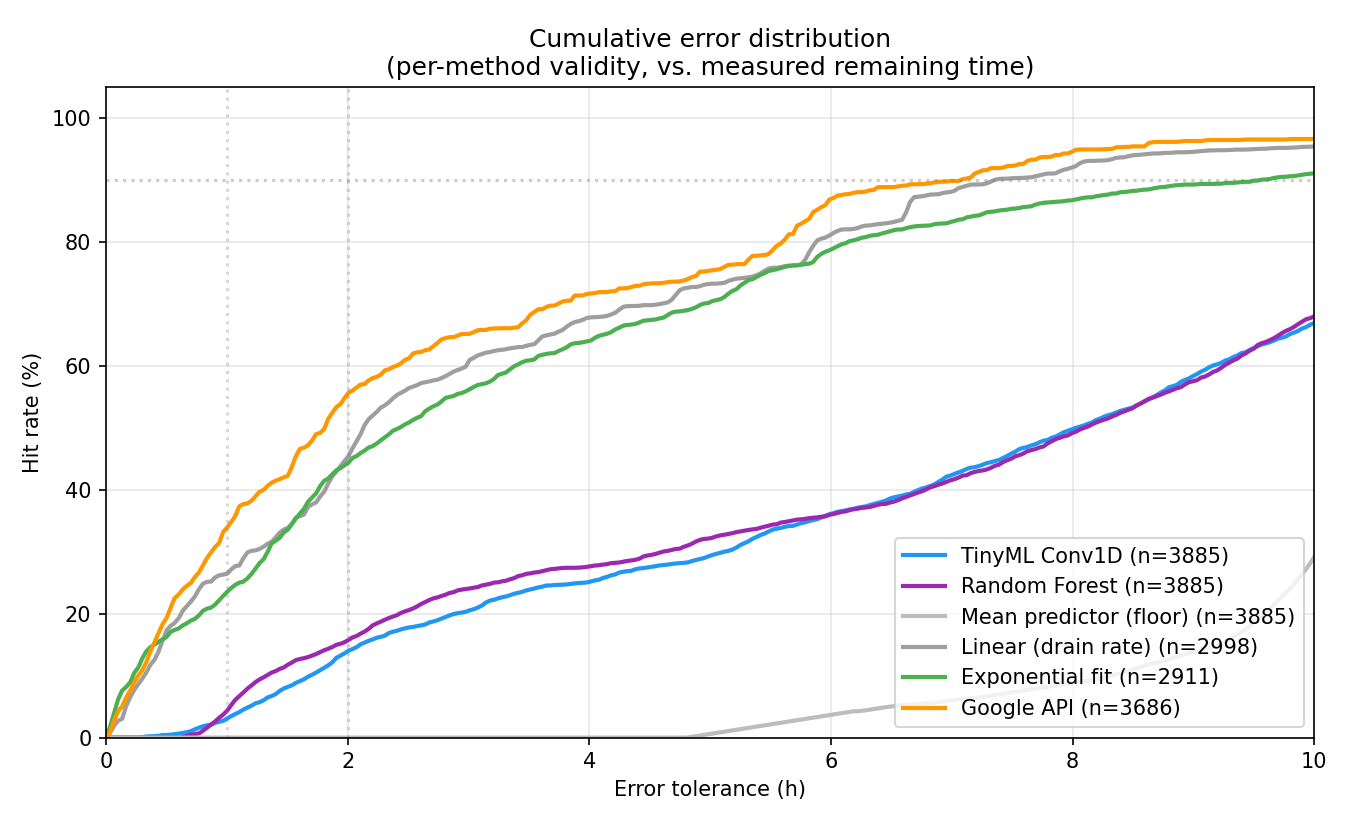
\includegraphics[width=0.85\linewidth]{cumulative_error.png}
\caption{Kumulative Fehlerverteilung der sechs verglichenen
Methoden auf dem leakage-freien Test-Set
($n{=}2{,}827$). Die x-Achse ist die Fehlertoleranz
in Stunden, die y-Achse der Anteil der Vorhersagen
innerhalb dieser Toleranz.}
\label{fig:cumulative}
\end{figure}

\newpage

% ████████████████████████████████████████████████████████████
%  6  DATENSCHUTZ
% ████████████████████████████████████████████████████████████
\section{Datenschutz}
\label{sec:datenschutz}

\subsection{Was wird erhoben?}

Die App speichert ausschließlich technische Geräte-Metriken (siehe
Datenmodell). Es gibt \emph{keinen} Zugriff auf:

\begin{itemize}
\item Standort (keine \code{ACCESS\_*\_LOCATION}-Permission)
\item Kontakte, Anrufprotokolle, SMS
\item Mikrofon, Kamera
\item Inhalte von Apps (kein Accessibility-Service, kein
  Screen-Recording)
\item Personenbezogene Identifikatoren wie IMEI oder Telefonnummer
\end{itemize}

Das einzige potenziell sensible Feld ist
\code{active\_app\_category}, und auch das nur als \emph{Kategorie}
(0--5), nicht als konkreter Paketname.

\subsection{Wo wird gespeichert?}

Im internen Verzeichnis der App (\code{Context.filesDir}):

\begin{itemize}
\item Nur diese App selbst hat Zugriff.
\item Andere Apps können nichts lesen (Android-Sandbox).
\item Bei Deinstallation werden die Daten automatisch mit entfernt.
\item Wird nicht in iCloud / Google Backup synchronisiert.
\end{itemize}

\subsection{Export}

Nur über expliziten Nutzerklick (Share-Intent). Es gibt
\emph{keinen} automatischen Upload, keinen Server, keine
Telemetrie. Der Nutzer entscheidet, ob die CSV per Mail, Drive oder
USB-Kabel weitergegeben wird.

\subsection{Berechtigungen}

\begin{table}[H]
\centering
\caption{Im Manifest deklarierte Permissions}
\label{tab:permissions}
\small
\begin{tabular}{lp{8.5cm}}
\toprule
\textbf{Permission} & \textbf{Wofür} \\
\midrule
\code{FOREGROUND\_SERVICE} & Background-Service mit Notification \\
\code{FOREGROUND\_SERVICE\_SPECIAL\_USE} & Service-Typ ab Android 14 \\
\code{WAKE\_LOCK} & Service läuft auch bei Display aus \\
\code{RECEIVE\_BOOT\_COMPLETED} & Auto-Restart nach Geräte-Neustart \\
\code{ACCESS\_NETWORK\_STATE} & WiFi-/Mobile-Daten-Status lesen \\
\code{ACCESS\_WIFI\_STATE} & WiFi-Status, Hotspot-Reflection \\
\code{PACKAGE\_USAGE\_STATS} & Aktive App lesen (Nutzer muss manuell aktivieren) \\
\code{POST\_NOTIFICATIONS} & Vorhersage in Notification anzeigen \\
\code{REQUEST\_IGNORE\_BATTERY\_OPTIMIZATIONS} & Service vor Doze schützen \\
\bottomrule
\end{tabular}
\end{table}

\subsection{Beim Verteilen an Mitstudierende}

Für die drei Pixel-Geräte habe ich die App-APK per E-Mail
verschickt. Vor der Installation wurde den drei Personen erklärt:

\begin{itemize}
\item welche Daten gesammelt werden (CSV mit 14 Spalten),
\item wo sie lokal liegen (nur auf ihrem Phone),
\item dass die CSV nur zu mir kommt, wenn sie sie aktiv per
  Share-Intent verschicken,
\item dass keinerlei Auto-Upload oder Hintergrund-Übertragung
  stattfindet.
\end{itemize}

Eine schriftliche Einwilligung hat jeder per WhatsApp bestätigt.

\newpage

% ████████████████████████████████████████████████████████████
%  7  KI-NUTZUNG
% ████████████████████████████████████████████████████████████
\section{KI-Nutzung}
\label{sec:ki}

Während des Projekts habe ich \textbf{Claude Code} (Anthropic, Modell
Opus~4.7 mit 1M-Token-Kontext) als Programmier-Assistent verwendet.
Dieser Abschnitt ist bewusst transparent gehalten.

\subsection{Wofür Claude genutzt wurde}

\begin{itemize}
\item \textbf{Code-Refactoring:} Umstrukturierung von einem
  monolithischen Trainings-Skript zu einer modularen Pipeline
  (\code{methods/}, \code{evaluation/}).
\item \textbf{Boilerplate:} TFLite-Konvertierungs-Boilerplate,
  Argument-Parser, Standard-Plot-Code (matplotlib).
\item \textbf{Methodische Recherche:} Suche nach relevanter
  Literatur (Li 2018, Albelali \& Ahmed 2025, Flores-Martin 2024,
  MLPerf~Tiny, Harrell 1982).
\item \textbf{Statistische Tests:} Implementierung des
  Concordance-Index, Bootstrap-Konfidenzintervalle und
  Permutationstests nach meinen Vorgaben.
\item \textbf{Paper-Schreibhilfe:} Strukturierung des LaTeX-Papers,
  Tabellen-Formatierung, Korrektur-Lesen.
\item \textbf{Mehrere Audit-Runden:} Die KI hat geholfen, eigene
  Fehler (falsche Quellen-Autoren, inkonsistente Zahlen,
  methodische Schwächen wie den Hardware-vs.\,Datenverteilungs-
  Confounder) systematisch zu finden.
\end{itemize}

\subsection{Was ich selbst gemacht habe}

\begin{itemize}
\item Das gesamte Projekt-Konzept und die Forschungsfrage.
\item Auswahl der zehn Features (auf welche APIs man als App
  zugreifen kann).
\item Datensammlung auf den vier Geräten -- inklusive
  App-Verteilung an Mitstudierende.
\item Alle methodischen Entscheidungen: Segment-Level-Split,
  C-Index als Metrik, Wahl der Vergleichsmethoden, Bucket-Analyse.
\item Kritisches Hinterfragen der KI-Vorschläge, wenn etwas
  methodisch verdächtig wirkte. Im Verlauf entdeckte die KI auf
  Nachfrage mehrere eigene Fehler, etwa falsche Autoren bei drei
  Quellen, erfundene Bucket-Zahlen und zu plakative Aussagen wie
  \glqq{}Linear = Google\grqq{}.
\item Alle Anpassungen am Android-Manifest, Permissions,
  geräte-spezifisches Debugging (MIUI-Service-Stirbt-Problem).
\end{itemize}

\subsection{Bilanz}

Realistisch eingeschätzt: ohne KI-Unterstützung hätte ich das
Projekt in dieser Tiefe nicht in sieben Wochen geschafft. Die KI
war besonders nützlich für \emph{Boilerplate und
Recherche-Beschleunigung} sowie für \emph{methodische Disziplin}
(Audit-Pass, Konsistenz-Checks über große Code-Mengen).

Was die KI \emph{nicht} ersetzt hat: die Entscheidung, was gemacht
wird, das Verstehen der Ergebnisse, die Verteidigung von
Trade-offs, und vor allem die handfeste Geräte-Logistik und das
Debugging vor Ort.

\newpage

% ████████████████████████████████████████████████████████████
%  8  ERFAHRUNGSBERICHT
% ████████████████████████████████████████████████████████████
\section{Wöchentlicher Erfahrungsbericht}
\label{sec:wochenbericht}

\subsection*{Woche 1 (KW 13: 23.--29.\,März)}

\textbf{Setup und erste Datensammlung.}
Repo angelegt, Android-Projekt aufgesetzt, erste Version des
\code{DataCollectorService} geschrieben. Schon am 25.\,März lief
die erste Messung auf dem Xiaomi durch. Hauptproblem in dieser
Woche: die \code{PACKAGE\_USAGE\_STATS}-Permission ist nicht via
Standard-Dialog vergebbar -- der Nutzer muss in den Einstellungen
manuell ankreuzen. Ich habe deshalb einen Button in der App
eingebaut, der direkt zum \code{ACTION\_USAGE\_ACCESS\_SETTINGS}
springt.

\subsection*{Woche 2 (KW 14: 30.\,März -- 5.\,April)}

\textbf{Service-Robustheit.}
Datensammlung bricht beim Wegwischen aus der App-Übersicht ab.
Drei Tage damit verbracht herauszufinden, wie man auf
Xiaomi-MIUI einen Service vor dem Aggressive-Killing schützt.
Lösung: \code{onTaskRemoved} $\to$
\code{AlarmManager.setExactAndAllowWhileIdle} $\to$ Service kommt
1 Sekunde später wieder. Plus \code{BootReceiver} damit nach
Neustart automatisch weitergesammelt wird.

\subsection*{Woche 3 (KW 15: 6.--12.\,April)}

\textbf{Erstes Modell, erste Auswertung -- erstes Erschrecken.}
Genug Daten zusammen ($\sim$11.000 Messpunkte), erstes Training
durchgelaufen, MAE 0.53\,h. Habe das stolz aufgeschrieben. Dann
stutzig geworden: warum ist das so viel besser als die
Google-API? Beim Nachprüfen festgestellt, dass das ein klassisches
Data-Leakage-Artefakt vom Random-Split war. Pipeline auf
Segment-Level-Split umgestellt $\to$ MAE wird zu 9.96\,h. Das war
der methodische Wendepunkt der Arbeit.
Am 12.\,April App-APK an einen Mitstudierenden mit Pixel~7~Pro
weitergegeben.

\subsection*{Woche 4 (KW 16: 13.--19.\,April)}

\textbf{Multi-Device wird real.}
APK an zwei weitere Pixel-Nutzer verteilt (Pixel~8~Pro,
Pixel~9~Pro~XL). Schwierig vor allem die Aufklärung darüber, was
genau gesammelt wird -- ich habe einen Mini-Datenschutz-Hinweis
schriftlich verschickt und mündlich erklärt. Alle drei haben
zugestimmt. Parallel das CSV-Schema erweitert
(\code{system\_personalized}, \code{linear\_baseline\_h}) und den
Logger so gebaut, dass er bei Schema-Wechsel die alte Datei
sicher parkt.

\subsection*{Woche 5 (KW 17: 20.--26.\,April)}

\textbf{Auswertungs-Tiefe.}
Pipeline so umgebaut, dass sie alle vier Geräte-CSVs konsolidiert
und auswertet. Mean-Predictor und Random Forest als
Sanity-Modelle hinzugefügt, weil ein
\glqq{}TinyML schlägt nichts\grqq{} wenig aussagekräftig wäre,
ohne zu zeigen womit es überhaupt verglichen wird. Dazu noch die
analytischen Baselines (Linear, Exponential) implementiert.

\subsection*{Woche 6 (KW 18: 27.\,April -- 3.\,Mai)}

\textbf{Statistische Härte.}
Bootstrap-Konfidenzintervalle, Permutationstests,
modell-unabhängige Feature-Diagnose (Pearson, Spearman, Mutual
Information). Zwischendurch die Xiaomi-Datensammlung beendet
(28.\,April) -- die finale Datenmenge stand fest: 66.001
Messpunkte. Erkenntnis dieser Woche: TinyML schlägt auf
Multi-Device den Mean-Predictor signifikant ($p \leq 0.005$) --
anders als noch auf Single-Device, wo es statistisch indifferent
war.

\subsection*{Woche 7 (KW 19: 4.--11.\,Mai)}

\textbf{Konsolidierung und Paper-Schreiben.}
Pixel-Datensammlung beendet (10.\,Mai). Per-Device-Analyse zeigt
sehr unterschiedliche Performance pro Gerät -- auf Pixel~7~Pro
$C{=}0{.}79$, auf Xiaomi nur $0{.}59$. Datenverteilungs-Confounder
identifiziert: auf Xiaomi war der Akku 88\,\% der Zeit über
75\,\%, weshalb wenig Discharge-Dynamik zum Lernen da war.
Diese Woche viel Zeit darin investiert, dass das Paper methodisch
sauber formuliert ist und die Quellen wirklich das sagen, was
zitiert wird (zwei Quellen-Audits, vier korrigierte
Autorenangaben, eine korrigierte Größenordnung-Behauptung).

\subsection{Aufwand}

\begin{table}[H]
\centering
\caption{Zeitaufwand nach Woche}
\label{tab:aufwand}
\small
\begin{tabular}{lp{9cm}r}
\toprule
\textbf{Woche} & \textbf{Hauptaufwand} & \textbf{Stunden} \\
\midrule
1 & App-Grundgerüst + Permissions                  & $\sim$\;15 \\
2 & Service-Robustheit auf MIUI                    & $\sim$\;18 \\
3 & Trainings-Pipeline + Leakage-Aha-Moment        & $\sim$\;20 \\
4 & Schema-Migration + APK-Verteilung              & $\sim$\;10 \\
5 & 6-Wege-Vergleich + analytische Baselines       & $\sim$\;18 \\
6 & Statistische Tests + Daten-Diagnose            & $\sim$\;15 \\
7 & Paper schreiben + Audits + Verteidigung        & $\sim$\;25 \\
\midrule
\textbf{Summe} & & \textbf{$\approx$\,120\,h} \\
\bottomrule
\end{tabular}
\end{table}

\newpage

% ████████████████████████████████████████████████████████████
%  9  KURZREFERAT
% ████████████████████████████████████████████████████████████
\section{Kurzreferat-Folien}
\label{sec:folien}

Für die mündliche Verteidigung habe ich eine 16-Folien-Präsentation
unter \datei{paper/Verteidigung.pptx} erstellt. Sie deckt ab:

\begin{enumerate}
\item Titel und Forschungsfrage
\item Motivation (Settings-App vs.\ Google-API seit Android~12)
\item Verwandte Arbeiten
\item Datensammlung: 4 Geräte, 45 Tage
\item Sechs verglichene Methoden
\item Methodik-Kernpunkt: Segment-Level-Split
\item Hauptergebnisse (6-Wege-Vergleich)
\item Statistische Signifikanz (Permutationstests)
\item Per-Device-Analyse (Hardware-Effekt)
\item Effizienz-Benchmark (TFLite-Quantisierung)
\item Diskussion: TinyML lernt Signal
\item Diskussion: Google\,$\approx$\,Linear-Baseline
\item Limitations
\item Conclusion (drei Achsen)
\item Q\&A
\end{enumerate}

Die Folien sind absichtlich für die wissenschaftliche
Paper-Verteidigung optimiert. In diesem Portfolio-Kontext
(App-Entwicklungs-Fokus) wären andere Schwerpunkte sinnvoll
(Service-Lifecycle, App-Verteilungs-Erfahrung, Geräte-Logistik).
Falls ein eigenes Portfolio-Kurzreferat verlangt wird, kann ich
daraus eine angepasste Variante extrahieren.

% ████████████████████████████████████████████████████████████
%  10  ZUSAMMENFASSUNG
% ████████████████████████████████████████████████████████████
\section{Zusammenfassung}
\label{sec:zusammenfassung}

\subsection[Was funktioniert (Stand 11.\ Mai 2026)]{Was funktioniert (Stand 11.\,Mai 2026)}

\begin{itemize}
\item Android-App läuft stabil im Hintergrund auf vier
  verschiedenen Geräten über mehrere Wochen.
\item TFLite-Modell ist 14.4\,KB groß, läuft auf der CPU des
  Phones in $\sim$\,5\,$\mu$s pro Inferenz.
\item Datensammlung umfasst 66.001 Messpunkte, sauber per
  Share-Intent exportiert.
\item Trainings- und Auswertungs-Pipeline reproduzierbar via einem
  Befehl (\code{python run\_pipeline.py}).
\item Wissenschaftliches Paper erstellt (separates Dokument).
\end{itemize}

\subsection{Was noch nicht ideal ist}

\begin{itemize}
\item Die App-UI ist zweckmäßig, aber nicht hübsch. Material-3 ist
  nur das Default-Theme.
\item Die Scaler-Werte werden manuell aus dem Python-Modell ins
  Kotlin kopiert -- automatisierbar via Build-Step wäre eleganter.
\item Es gibt kein In-App-Onboarding für die UsageStats-Permission,
  nur einen Button-Hinweis.
\end{itemize}

\subsection{Was ich aus dem Projekt mitnehme}

\begin{itemize}
\item \textbf{Android im Hintergrund ist hart.} Theoretisch sind
  Foreground-Services eine Standard-Lösung. Praktisch killt jeder
  Hersteller anders. Multi-Device-Test ist die einzige
  Möglichkeit, das wirklich zu prüfen.
\item \textbf{Methodische Disziplin schlägt Modell-Komplexität.}
  Der Wechsel von Random-Split zu Segment-Level-Split hatte mehr
  Einfluss auf das Ergebnis als jedes Hyperparameter-Tuning.
\item \textbf{Negative Ergebnisse ehrlich darstellen ist genau so
  wertvoll wie positive.} Anfangs schien das Projekt zu
  \glqq{}funktionieren\grqq{} (MAE 0.5\,h). Erst durch saubere
  Methodik kam heraus: TinyML funktioniert, aber nicht so
  spektakulär wie auf den ersten Blick. Das ehrlich aufzuschreiben
  ist anstrengender, aber wissenschaftlich korrekter.
\end{itemize}

\vfill

\begin{center}
\rule{0.6\linewidth}{0.4pt}\\[0.5em]
{\small Repository: \url{https://github.com/Keno-fsdf/HandyUsageRepo}}\\[0.3em]
{\small Eingereicht am \emph{12.\,Mai 2026} -- Keno Schürger}
\end{center}

\end{document}
